\section{R2U2 Software Implementation in Python}
While R2U2 is designed to be an online, embedded runtime monitor, it can often be useful to verify a trace offline. The Python implementation of R2U2 allows one to use R2U2's verification abilities offline as a fast and efficient way to verify a trace or validate an atomic formula over a trace.

\subsection{Getting Started}
Note that the following must be installed in order to use the Python implementation of R2U2:
\begin{itemize}
	\item Python 3.6 (or greater)
	\item \textbf{Python Packages:} argparse, py, random, logging, sys, collections
\end{itemize}
The Python implementation of R2U2 also runs from a UNIX based command line interface (CLI). Additionally, there are several types of input files users may use: 
\begin{itemize}
	\item \textbf{Input File:} There are two options for this input: an \textit{Assembly File} or a \textit{MLTL Formula}. The details and an example of each these formats will be discussed in Section \ref{InputFiles}.
	\item \textbf{Trace File:} There are two formats that this version of R2U2 will accept: a \textit{Sensor Input File} or an \textit{Atomic Input File}. The details and an example of each of these formats will be discussed in Section \ref{TraceFiles}.
	\item \textbf{Output File:} The name of the output file from R2U2. Note that if this is left blank, the default output file's name will be \textit{untitled.txt}.
\end{itemize}

\subsection{File Formats}
Note that user must provide an Input File and a Trace File to run R2U2, though there is no restrictions on the combination of these files. The Input File specifies the temporal logic formulas over which the atomic propositions are reasoned over. The Trace File is the atomics or sensor values that are being reasoned over.

\subsubsection{Input File Formats}
\label{InputFiles}
There are two different formats in which the temporal logic formulas can be entered into the Python version of R2U2: (1) \textbf{Assembly File} or (2) \textbf{MLTL Formula}.

\subparagraph{Assembly File:}
\label{AssemblyFile}
Like any other assembly file, this file is a list of single command instructions that R2U2 will execute, in order. An example of a R2U2 compatible Assembly File can be seen in Table \ref{FileTable}. Each line contains an instruction, which consists of a label, a command, and one or more variables/labels. The list of assembly commands the Python version of R2U2 can use is:
\begin{itemize}
	\item \textbf{\textit{load}:} Used to load the atomic from either the Sensor Input File or Atomic Input File. 
	\item \textbf{\textit{not}:} Used to denote the logical \textit{Negation} of an atomic.
	\item \textbf{\textit{and}:} Used to denote the logical \textit{AND} of two atomics.
	\item \textbf{\textit{until}:} Used to denote the \textit{Until} temporal logic function. This function takes in four arguments: the first is the label for the left-side of the \textit{Until}, the second is the right-side, the third is the relative start time, and the fourth is the relative end time.
	\item \textbf{\textit{boxbox}:} Used to denote the \textit{Global} temporal logic function. Assumes that the time bound starts at zero. First argument is the label (either atomic or instruction), the second is the relative end time of the function.
	\item \textbf{\textit{boxdot}:} Used to denote the \textit{Global} temporal logic function. First argument is the label (either atomic or instruction), the second is the relative start time of the function, and the third is the relative end time of the function.
	\item \textbf{\textit{end}:} Used to denote the end of the assembly file. This command must be at the end of the Assembly File and its argument must be the second-to-last label.
\end{itemize}

\begin{table}[H]
	\caption{Examples of the format for the Input Files}
	\label{FileTable}
	\begin{center}
	\begin{tabular}{l | l}
		\hline
		\hline
		\textbf{File Type} & \textbf{Assembly File}\\
		\hline
		line 1 & s0: load a0\\
		line 2 & s1: load a1\\
		line 3 & s2: not a0\\
		line 4 & s3: not a1\\
		line 5 & s4: and a0 a1\\
		line 6 & s5: and s2 s3\\
		line 7 & s6: not s5\\
		line 8 & s7: until s7 s5 0 3\\
		line 9 & s8: boxbox s8 3\\
		line 10 & s9: end s8\\
		\hline
		\hline
	\end{tabular}
	\end{center}
\end{table}

\subparagraph{MLTL File:}
\label{MLTLFile}
When one, complex function is to be evaluated, a user may find it easier to generate a MLTL File, or enter the function directly via the CLI, rather than manually create the assembly code. The valid expressions for an MLTL formula are given in Table \ref{MLTLCommands}.

\begin{table}[H]
	\caption{The format for the MLTL formulas, either in a single line of a text file or via the CLI. Note that $E$1 and $E$2 denote that that parameter can be either an expression, to allow for more complex formulas, or a single atomic.}
	\label{MLTLCommands}
	\begin{center}
	\begin{tabular}{l | c | c}
		\hline
		\hline
		\textbf{Expression} & \textbf{Syntax} & \textbf{Precedence} \\
		\hline
		\textit{NOT} & !$E$1 & 1\\
		\textit{Next} & $XE$1 & 1\\
		\textit{Until} & $E$1 $U$[$t_i$,$t_f$] $E$2 & 2\\
		\textit{Until} & $E$1 $U$[$t_f$] $E$2 & 2\\
		\textit{Global} & $G$[$t_i$,$t_f$] $E$1 & 2\\
		\textit{Global} & $G$[$t_f$] $E$1 & 2\\
		\textit{AND} & $E$1 \& $E$2 & 3\\
		\textit{OR} & $E$1 $|$ $E$2 & 3\\
		\hline
		\hline
	\end{tabular}
	\end{center}
\end{table}

Note that precedence can be overruled using parenthesis or brackets. Additionally all tuple time stamps must be comma separated. The following is an example of a complex MLTL formula and its syntactical conversion into a command that the Python version of R2U2 can reason over:

\begin{equation}
G_{0,5}(\neg{a_0}U_{0,3} (a_1 \bigwedge a_2)) \bigvee \neg{Xa_0} \rightarrow ((G[5] ((!a0) U[0,3] (a1 \& a2))) | !(Xa0)
\label{ExampleMLTL}
\end{equation}

\subsubsection{Trace File Formats}
\label{TraceFiles}
The two Trace File formats are given in Table \ref{SensorFileTable}. Note that the two formats require the first line to be a label, either that of the sensor or the atomic. In order for the tool to parse the input file,  values in this file must be separated by a space or a comma. Each line is an increment in time, starting at time $t=0$.

\subparagraph{Sensor Input File:}
\label{SensorInputFile}
The values of the sensor input file can be either signed/unsigned integers, single/double precision floating point, or hexadecimal values. Since R2U2 reasons over boolean values, these sensor values must be converted to a boolean value by performing some type of conditional reasoning, i.e., $=$, $\neq$, $>$, $<$, $\geq$, $\leq$. To do this, the \textit{Traverse.py} file, located in the \textbf{R2U2\_SW/R2U2\_PYTHON/ACOW} directory, must be modified. Specifically the \textbf{def s2a} function maps the sensor functions into boolean atomics. Note that Fig.\ref{fig:sa} shows the formatting for how to perform the boolean mapping.
\begin{center}
	\begin{figure}[H]
		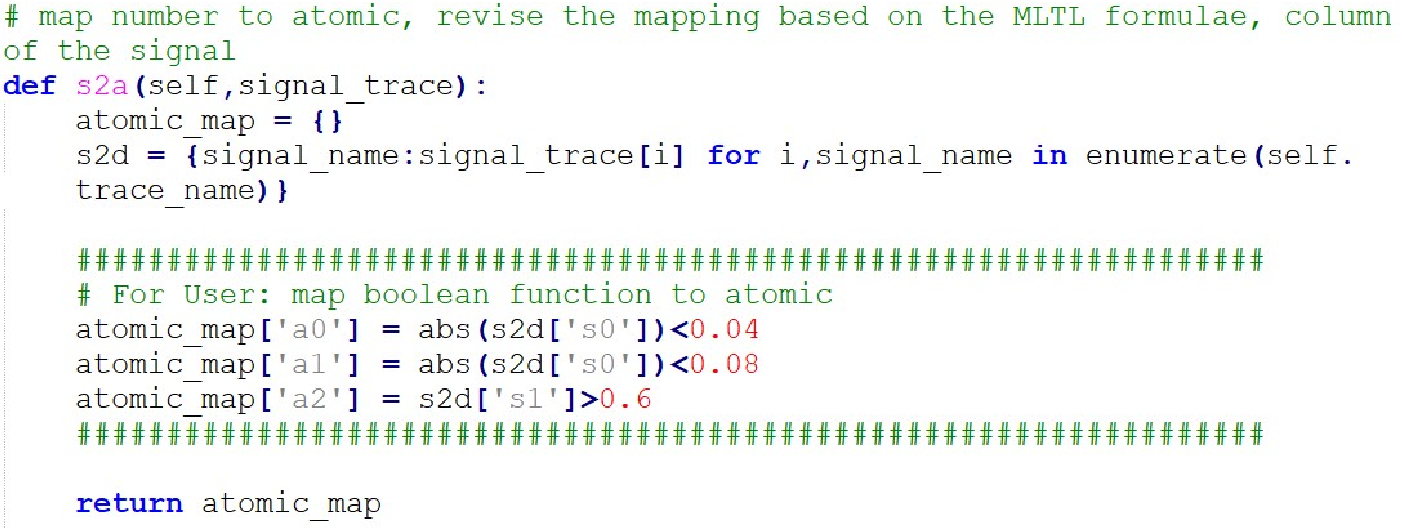
\includegraphics[scale=0.5]{fig/TraverseScreenshot.pdf}
		\caption{A screenshot of the \textbf{s2a} function within the \textit{Traverse.py} file. Note that this function must be modified in order to convert the sensor values into boolean atomics.}
		\label{fig:sa}
	\end{figure}
\end{center}

\subparagraph{Atomic Input File:}
\label{AtomicInputFile}
The values of the atomic input file must be Booleans, i.e., a $0$ or $1$. Unlike the sensor input file, there is no need to modify the \textit{Traverse.py} file when using this version of an input file. An example of the format can be seen in Table \ref{SensorTable}.

\begin{table}[H]
	\caption{Examples of the format for the Trace Files}
	\label{SensorTable}
	\begin{center}
	\begin{tabular}{l | ccc | ccc}
		\hline
		\hline
		\textbf{File Type} & \multicolumn{3}{c|}{\textbf{Sensor Input File}} & \multicolumn{3}{c}{\textbf{Atomic Input File}}\\
		\hline
		Line \# & Sensor 0 & Sensor 1 & $\dots$ & Atomic 0 & Atomic 1 & $\dots$\\
		\hline
		line 1 & Altitude & Velocity & $\dots$ & a0 & a1 & $\dots$\\
		line 2 & 1005 & 10.0 & $\dots$ & 0 & 0 & $\dots$\\
		line 3 & 1011 &  9.8 & $\dots$ & 1 & 0 & $\dots$\\
		line 4 & 1015 & 10.4 & $\dots$ & 1 & 1 & $\dots$\\
		line 5 & $\vdots$ & $\vdots$ & $\ddots$ & $\vdots$ & $\vdots$ & $\ddots$\\
		\hline
		\hline
	\end{tabular}
	\end{center}
\end{table}

\subsection{CLI Overview}
To use the Python version of R2U2, navigate to the \textbf{R2U2\_SW/R2U2\_PYTHON/} directory within a UNIX bash terminal. Verify your current version of Python by entering \textbf{python3 --version}. If your current version is Python 3.6 or greater, proceed. If not, you must install Python 3 to continue.

The command structure for running R2U2 is as follows:
\begin{lstlisting}[language=Bash]
	python MLTL_main.py -m "$(cat [A])" -s [B] -o [C]
\end{lstlisting}
where \textbf{[A]} is the path and name of Input File, \textbf{[B]} is the path and name of Trace File, and \textbf{[C]} is the name of the Output File. Remember that \textbf{[C]} is optional, and if it is not specified, then the default output file name is \textit{untitled.txt}. Note that if the user wishes to manually enter a MLTL formula into the command line, rather than use an input file, then the ``\$(cat [A])'' can be replaced with the MLTL formula.

\clearpage
